%% LyX 2.0.0 created this file.  For more info, see http://www.lyx.org/.
%% Do not edit unless you really know what you are doing.
\documentclass[english]{article}
\usepackage[T1]{fontenc}
\usepackage[utf8]{luainputenc}
\usepackage{graphicx}

\makeatletter

%%%%%%%%%%%%%%%%%%%%%%%%%%%%%% LyX specific LaTeX commands.
%% Because html converters don't know tabularnewline
\providecommand{\tabularnewline}{\\}

%%%%%%%%%%%%%%%%%%%%%%%%%%%%%% User specified LaTeX commands.
\makeatother

\makeatother

\usepackage{babel}
\begin{document}

\title{Performance Report on EC2 Instances}


\author{Vineet Kumar, Phuc Xuan Nguyen}

\maketitle

\section{Introduction}

Amazon Elastic Compute Cloud(EC2) is a web service that provides resizable
computing power through the cloud. There are lots of disputes online
regarding the correctness of the {}``rated'' hardware performance
of Amazon EC2. Some articles claims that the actual performance of
the hardware is much less than the advertised number. We are interested
in testing to see whether such claim is accurate, and if not, what
the reason might be. As a later part of the project, we are also interested
in the overhead of the linux containers(LXC) on a virtualized platform. 

The aim of this project is to measure performance on Amazon's EC2
instances. For the first portion of this project we measure the overhead
of CPU, scheduling and OS services. All the code for our tests was
written in C. We used gcc 4.6.1 with no optimizations to run our code.
Collecting machine description information, measuring procedure call
overhead and measurment overhead were done by Phuc Xuan Nguyen. Measurement
of system call overhead, process creation, kernel thread creation,
process context switch and kernel context switch were done by Vineet
Kumar. We think we spent in total of around 7 working days for this
portion of the project.


\section{Machine Description}

We are aiming to measure the performance on the Amazon's t1.micro
instances. 
\begin{itemize}
\item 1 Elastic Computing Unit 
\item Processor: Intel(c) Xeon(R) CPU E5430 @ 2.66Ghz.

\begin{itemize}
\item 12M L2 Cache, 1333 Mhz FSB 
\end{itemize}
\item Memory: 592MiB 
\item Netword card speed

\begin{itemize}
\item Between EC2 Instances: 100MB/s 
\end{itemize}
\item Disk: Amazon Elastic Block (EBS)

\begin{itemize}
\item Size: 7.9GB 
\end{itemize}
\item Operating System: Ubuntu Oneric 11.10 
\end{itemize}

\section{CPU Operation}

For all our experiments we use RDTSC counter. To obtain time we divide
this by the CPU frequency. Also of all the data seen, we discard the
best and worst 10\% of data and then take mean values.


\subsection{Measurement overhead}


\subsubsection{Experiment}

We are using RDTSC as a fine-grained counter to measure the performance.
In order to calculate the overhead of RDSTC, we run the following
experiment.

Function 1: 
\begin{itemize}
\item Get initial clock counter 
\item Repeat N times:

\begin{itemize}
\item Run RDTSC 
\item Perform a random function f 
\end{itemize}
\item Return the difference between the current and the initial clock counter. 
\end{itemize}
Function 2: 
\begin{itemize}
\item Get initial clock counter 
\item Repeat N times:

\begin{itemize}
\item Perform a random function f 
\end{itemize}
\item Return the difference between the current and the initial clock counter
\end{itemize}
To measure the for loop overhead, we set up two procedures: (1) using
a for loop to execute a function foo() 50 times, and (2) just execute
foo() 50 times in a row. Through experiment we find that the amount
of times does not affect the interested results.


\subsubsection{Results}

We find that the variance becomes insignificant when N is around 10000.
We avoid the possible compiler optimization by running the random
function f.

We calculate the difference in the result of Function 2 and Function
1 and divide that by N to find the overhead of RDTSC. In the t1.micro
instance.
\begin{itemize}
\item Without RDTSC: average 6.00 cycles \textasciitilde{} 2.25 $\mu s$
\item With RDTSC: average 48 cycles \textasciitilde{} 18.04 $\mu s$
\item The overhead of RDSTC: \textasciitilde{} 15.789$\mu s$
\end{itemize}
After running the for-loop experiment 10000 times, we find that
\begin{itemize}
\item Without for loop: average 12.6 cycles \textasciitilde{} $4.7\mu s$
\item With for loop: average 21.8 cycles \textasciitilde{} $7.89\mu s$
\end{itemize}
So the overhead of the for loop is the difference between these, which
is around 9.2 cycles \textasciitilde{} $3.38\mu s$.


\subsection{Procedure call overhead}

To find out the procedure call overhead, we perform two simple operations
(int x = 1+1; int y = x;) in 9 different scenarios: no procedure call
and procedure calls with the 0-7 parameters. Figure ? describes the
increment in overhead.

The result, gathered after running 1,000,000 iterations, is shown
in Figure 1.

\begin{figure}
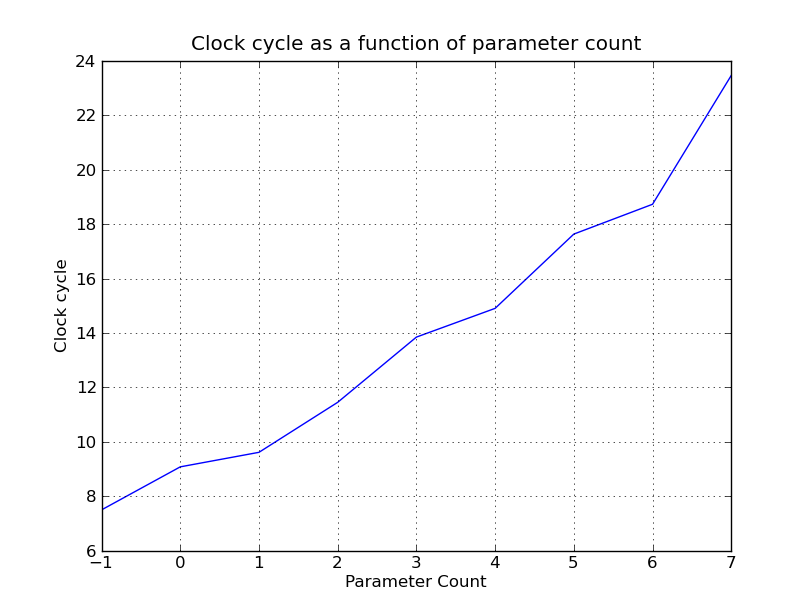
\includegraphics[scale=0.5]{procedure_call_result}\caption{Clock cycle(param){*} -1 means no procedure call}
\end{figure}



\subsection{System call overhead}
\begin{enumerate}
\item Prediction - System Call is a slightly heavier call than a simple
procedure call, it needs to do more checks and in effect is the only
domain crossing for our system. Thus we predict that system call overhead
time would be little more than a procedure call. Its hard to make
other predictions for a system call.
\item Experiment: To measure system call overhead, we need to do measurements
on a system call that does not do much work. We do our experiments
by calling {}``getpid()'' and by writing one byte to the device
devnull. We notice that for both these experiments if we run a tight
loop within a single process, the system call gets cached and thus
does not give us correct overhead measurements. Thus, we handle this
issue by running the test within a context of different process. We
run the test for 10,000 iterations. Table 1 shows the results:Results:
The following table shows the results:
\item Results :
\item 
\begin{table}
Table 1: System call overhead

\begin{tabular}{|c|c|c|c|c|}
\hline 
System Call  & Time - cached($\mu$s)  & Std. dev- cached  & Time - uncached($\mu$s)  & Std. dev - uncached\tabularnewline
\hline 
\hline 
getpid()  & 0.00358 (9.66 M cycles) & 1.71$\%$  & 7.89 (21303 M cycles) & 5.74\%\tabularnewline
\hline 
write to devnull  & 0.00341 (9.21 M cycles) & 1.06\%  & 1.45 (3915 M cycles) & 53\%\tabularnewline
\hline 
\end{tabular}
\end{table}

\item Analysis : We see that the time needed for a getpid() is slightly
more than a procedure call
\end{enumerate}

\subsection{Task creation time}

Prediction : We epect task creation to take much more time than a
system call, as it involves context switch when a new task needs to
created. We expect kernel thread creation to take less time as in
effect a user thread is tied to kernel.

We measure the task creation time by calling the timer before a fork()
is issued and immediately inside the child process. We repeat this
process for 10, 000 iterations. To measure the creation time for a
kernel thread - we use posix thread attributes to tie a user thread
to a kernel level thread. We repeat these experiments 10,000 times.
We use the following test methodology : 
\begin{enumerate}
\item Repeat N times 
\item Start timer 
\item Fork a process 
\item Stop timer inside the child process 
\end{enumerate}
\begin{table}
Table 2: Process and kernel thread creation overhead

\begin{tabular}{|c|c|c|}
\hline 
 & Time($\mu$s)  & Std. deviation\tabularnewline
\hline 
\hline 
Process creation  & 264.73(714771 M cycles)  & 18.48\%\tabularnewline
\hline 
Kernel Thread Creation  & 1.89 (5103 M cycles) & 35 \tabularnewline
\hline 
\end{tabular}
\end{table}


Analysis : Process creation time takes much longer than kernel thread
creation, a part of the explanation could be that process creation
needs to do domain crossing, whereas kernel thread creation does not.


\subsection{Context switching time}

Prediction : We expect context switch time to take atleast the time
needed for system call. 

We measure context switch time by passing a token across pipes. We
create a total of 4 pipes to accomplish a 2 way communication and
measure the round trip time. This roundtrip time per process contains
time needed to conext switch twice and time for a read and write call
using pipes. We however, do not remove the pipe overhead - that needs
to be done. We run our experiments for N iterations

This is the test methodology we use for measuring a process context
switch time 
\begin{enumerate}
\item Create 2 pipes for communication between process 1 and process 2 (pipe1) 
\item Create 2 pipes for communication between process 2 and process 1 (pipe2) 
\item Repeat N times

\begin{enumerate}
\item Start timer 
\item Repeat (c) -(d) for some iterations 
\item Process 1 writes to pipe1, process 2 reads it. Note that these will
be blocking reads. This causes Process 2 to start running 
\item Process 2 writes to pipe2 and process 1 reads it. This will again
cause a context switch 
\item Stop timer 
\end{enumerate}
\end{enumerate}
For Measuring kernel thread context switch time we use posix threads
bound to kernel by setting scope attribute to PTHREAD\_SCOPE\_SYSTEM
\begin{table}
Table 3: Context Switching overhead

\begin{tabular}{|c|c|c|}
\hline 
 & Time ($\mu$s)  & Std. deviation\tabularnewline
\hline 
\hline 
Process Context Switch  & 2.19 (5913 M cycles) & 27.8\%\tabularnewline
\hline 
Kernel thread context switch  & 2.65 (7155 M cycles) & 38.5\%\tabularnewline
\hline 
\end{tabular}
\end{table}
Analysis : Table shows that context switch time is of the order of
a system call, and that kenrel thread conext switch does not vary
much with process context switch time. 
\end{document}
